
\documentclass[hyperref={pdfpagelabels=false},ngerman]{beamer}

% stop font warning
\let\Tiny=\tiny
\providecommand\thispdfpagelabel[1]{}

\usepackage[english]{babel}
\usepackage{lmodern}
\usepackage[T1]{fontenc}
\usepackage[utf8]{inputenc}
\usepackage{graphicx,import}
\usepackage{stackengine}
\usepackage{feynmp}
\DeclareGraphicsRule{*}{mps}{*}{} 
\DeclareGraphicsExtensions{.pdf}
\usepackage{amsmath,amssymb,amstext,amsfonts} % mathrsfs
\usepackage{array,booktabs,tabularx}
\usepackage{tikz,tikz-uml,pgf-pie}
\usetikzlibrary{shapes,calc,arrows,positioning}
\tikzstyle{block} = [rectangle, draw, text width=7em, text centered, minimum height=2em]
\tikzstyle{arrow} = [draw, -latex, thick]
\tikzstyle{arrow2} = [draw, latex-latex, thick]
\tikzstyle{quark}  = [rectangle, draw, fill=yellow, minimum width=2em, text centered, minimum height=2em]
\tikzstyle{lepton} = [rectangle, draw, fill=red!50, minimum width=2em, text centered, minimum height=2em]
\tikzstyle{gauge}  = [circle   , draw, fill=green , minimum size=2em, inner sep=0pt, text centered]
\tikzstyle{scalar} = [diamond  , draw, fill=blue!40, minimum width=2.3em, text centered, minimum height=2.3em, inner sep=0pt]
\tikzstyle{goldstone} = [diamond, draw, dashed, fill=blue!30, minimum width=2.3em, text centered, minimum height=2.3em, inner sep=0pt]
\tikzstyle{squark}   = [diamond, draw, fill=yellow, minimum width=2.3em, text centered, minimum height=2.3em, inner sep=0pt]
\tikzstyle{slepton}  = [diamond, draw, fill=red!50, minimum width=2.3em, text centered, minimum height=2.3em, inner sep=0pt]
\tikzstyle{gaugino}  = [rectangle, draw, fill=green , minimum size=2em, inner sep=0pt, text centered]
\tikzstyle{higgsino} = [rectangle, draw, fill=blue!40  , minimum width=2em, text centered, minimum height=2em]
\tikzstyle{inert}    = [diamond  , draw, fill=teal!80, minimum width=2.3em, text centered, minimum height=2.3em, inner sep=0pt]
\tikzstyle{inertino} = [rectangle, draw, fill=teal!80, minimum width=2em, text centered, minimum height=2em]
\tikzstyle{phantom}  = [rectangle, minimum width=2em, text centered, minimum height=2em]
\usepackage{slashed}
\usepackage{fixltx2e} % textsubscript
\usepackage{multirow}
\usepackage{tcolorbox}
\usepackage{pifont}
\usepackage{xspace}
\usepackage{hyperref}
\hypersetup{colorlinks,linkcolor=,urlcolor=blue}
\usepackage{listings}
\lstset{breaklines=true,
  breakatwhitespace=true,
%  numbers=left,
  numberstyle=\tiny,
  stepnumber=1,
  basicstyle=\ttfamily\footnotesize,
  commentstyle=\ttfamily\color{gray},
  postbreak={\mbox{{$\hookrightarrow$}}\space\space},
  breakindent=10pt,
  breakautoindent=false,
  showspaces=false,
  showstringspaces=false,
  frame=single}

\definecolor{darkgreen}{RGB}{0,176,0}

\newcommand{\cmark}{\ding{51}}%
\newcommand{\xmark}{\ding{55}}%
\newcommand{\fmfvcenter}[1]{\;\vcenter{\hbox{\fmfreuse{#1}}}\;}
\newcommand{\eh}[1]{\,\mathsf{#1}}
\newcommand{\ok}{\textcolor{darkgreen}{\cmark}}
\newcommand{\notok}{\textcolor{red}{\xmark}}
\newcommand{\maybe}{\textcolor{gray}{\cmark}}
\newcommand{\meh}{\textcolor{gray}{\textbf{\huge\lower.1em\hbox{-}}}}
\newcommand{\Lagr}{\mathcal{L}}
\newcommand{\MS}{\ensuremath{M_S}}
\newcommand{\mathi}{\mathsf{i}}
\newcommand{\mycite}[1]{\ensuremath{\text{\textcolor{darkgray}{\tiny [#1]}}}}
\newcommand{\bigcite}[1]{\textcolor{darkgray}{[#1]}}
\newcommand{\dimrep}[1]{\mathbf{#1}}
\newcommand{\dimrepadj}[1]{\mathbf{\overline{#1}}}
\newcommand{\ESSM}{E\textsubscript{6}SSM}
\newcommand{\CESSM}{CE\textsubscript{6}SSM}
\DeclareMathOperator{\tildeRe}{\widetilde Re}
\DeclareMathOperator{\sign}{sign}
\DeclareMathOperator{\re}{Re}
\DeclareMathOperator{\im}{Im}
\renewcommand{\emph}{\textbf}
\newcommand{\dd}{\mathsf{d}}
\newcommand{\myurl}[1]{\href{#1}{#1}}
\newcommand{\Superpot}{\mathcal{W}}
\newcommand{\SuperField}[1]{#1}
\newcommand{\ConjSuperField}[1]{\bar{#1}}
\newcommand{\UY}{\ensuremath{U(1)_{Y}}}
\newcommand{\UN}{\ensuremath{U(1)_{N}}}
\newcommand{\Uem}{\ensuremath{U(1)_\text{em}}}
\newcommand{\SUL}{\ensuremath{SU(2)_\text{L}}}
\newcommand{\SUc}{\ensuremath{SU(3)_\text{c}}}
\newcommand{\SOten}{\ensuremath{{SO(10)}}}
\newcommand{\comma}{,}
\newcommand{\DRbar}{\ensuremath{\overline{\text{DR}}}}
\newcommand{\MSbar}{\ensuremath{\overline{\text{MS}}}}
\newcommand{\SM}{\ensuremath{\text{SM}}}
\newcommand{\SplitMSSM}{\ensuremath{\text{SM+split}}\xspace}
\newcommand{\SplitTHDM}{\ensuremath{\text{2HDM+split}}\xspace}
\newcommand{\MSSM}{\ensuremath{\text{MSSM}}}
\newcommand{\EFT}{\ensuremath{\text{EFT}}\xspace}
\newcommand{\THDM}{\ensuremath{\text{2HDM}}\xspace}
\newcommand{\hc}{\ensuremath{\text{h.c.}}}
\newcommand{\Qsplit}{\ensuremath{Q_\text{split}}\xspace}
\newcommand{\QTHDM}{\ensuremath{Q_\text{\THDM}}\xspace}
\newcommand{\Lag}{\ensuremath{\mathcal{L}}}
\newcommand{\pole}{\ensuremath{\text{pole}}}
\newcommand{\tree}{\ensuremath{\text{tree}}}
\newcommand{\fsstar}{\textbf{*}}
\newcommand{\Zv}{\ensuremath{\backslash\mkern-11.0mu{Z_3}}}
\newcommand{\downrightknickarrow}{\mathrel{\scalebox{1.3}{\rotatebox[origin=c]{180}{$\Lsh$}}}}
\newcommand{\threelinebrace}{$\left. \begin{array}{c} \\ \\ \\ \end{array} \right\rbrace$}
\newcommand{\fivelinebrace}{$\left. \begin{array}{c} \\ \\ \\ \\ \\ \end{array} \right\rbrace$}
\newcommand{\twolinebrace}{$\left. \begin{array}{c} \\ \\ \end{array} \right\rbrace$}
\newcommand{\elevenlinebrace}{$\left. \begin{array}{c} \\ \\ \\ \\ \\ \\ \\ \\ \\ \\ \\ \end{array} \right\rbrace$}
\newcommand{\at}{\alpha_t}
\newcommand{\ab}{\alpha_b}
\newcommand{\atau}{\alpha_\tau}
\newcommand{\as}{\alpha_s}

% threshold corrections HSSUSY:
\newcommand{\DlHSSUSY}[1]{\ensuremath{\Delta\lambda^{#1L}}}
% threshold corrections SplitMSSM:
\newcommand{\DlSplitMSSM}[1]{\ensuremath{\Delta\tilde{\lambda}^{\text{#1L}}}}
\newcommand{\gSplitMSSM}[1]{\ensuremath{\tilde{g}_{#1}}}
\newcommand{\DgSplitMSSM}[1]{\ensuremath{\Delta\tilde{g}_{#1}^{\text{1L}}}}
% threshold correction SplitMSSM-SM tower:
\newcommand{\DlSplitMSSMTower}{\Delta\lambda^{\text{\SplitMSSM--SM,1L}}}
% threshold correction THDM:
\newcommand{\DlTHDM}[2]{\Delta\lambda_{#1}^{\text{#2L}}}
% threshold correction SplitTHDMTHDMTower:
\newcommand{\DlSplitTHDM}[2]{\Delta\tilde\lambda_{#1}^{\text{#2L}}}
\newcommand{\gSplitTHDM}[1]{\ensuremath{\tilde{h}_{#1}}}
\newcommand{\gpSplitTHDM}[1]{\ensuremath{\tilde{h}_{#1}^{\prime}}}
\newcommand{\DlSplitTHDMTHDM}[2]{\Delta\lambda_{#1}^{\text{\SplitTHDM--\THDM,{#2}L}}}
% threshold correction SplitTHDMSplitTower:
\newcommand{\DgSplitTHDMSplit}[1]{\Delta\tilde{g}_{#1}^{\text{\SplitTHDM--\SplitMSSM,1L}}}

% set look of slides
\usetheme{Madrid}
\useoutertheme{default}
\useinnertheme{circles}
\usecolortheme{default}
\beamertemplatenavigationsymbolsempty % keine Navigationselemente
\setbeamersize{text margin left = 1cm, text margin right = 1cm}

% define footer
\makeatletter
\setbeamertemplate{footline}
{
  \hfill\hbox{\insertframenumber{} / \inserttotalframenumber\hspace*{4pt}}%
  \vskip3pt%
}
\makeatother
\usecolortheme{tud}

\title{Updates on Higgs mass predictions in FlexibleSUSY in the MSSM with different mass hierarchies}

\author[Alexander Voigt]{Emanuele Bagnaschi, \underline{Alexander Voigt}, Georg Weiglein\\[1em] [17xx.yyyyy]}

\date{KUTS-7, 17.07.2017}

\institute[Aachen]{RWTH Aachen}
\subject{FlexibleSUSY,MSSM,Higgs,EFT}
\keywords{FlexibleSUSY,MSSM,Higgs,EFT}

%%%%%%%%%%%%%%%%%%%%%%%%%%%%%%%%%%%%%%%%%%%%%%%%%%%%%%%%%%%%%%%%%%%%%%%%%%%%%

\begin{document}

%%%%%%%%%%%%%%%%%%%%%%%%%%%%%%%%%%%%%%%%
\begin{frame}[plain]
  \tikz [remember picture,overlay]
  \node at
    ([yshift=1.3cm,xshift=4cm]current page.south)
    {\includegraphics[height=2cm]{images/RWTH_Logo}};
  \titlepage  
\end{frame}

%%%%%%%%%%%%%%%%%%%%%%%%%%%%%%%%%%%%%%%%
\begin{frame}{Contents}
  \tableofcontents
\end{frame}

\section{Studied scenarios}

\begin{frame}{Contents}
  \tableofcontents[currentsection]  
\end{frame}

\begin{frame}{Scenarios with 1 light Higgs doublet}
  \begin{figure}
    \centering
    \stackunder[1em]{%
      \begin{tikzpicture}[scale=0.7, every node/.style={transform shape}]
        \node at (2,4) {MSSM};
        \draw (0,3) -- (4,3);
        \node at (2,2) {SM};
        \draw (0,1) -- (4,1);
        \node at (2,0) {SM(5)};
      \end{tikzpicture}
    }{\footnotesize{I high-scale SUSY}}\hfill
    \stackunder[1em]{%
      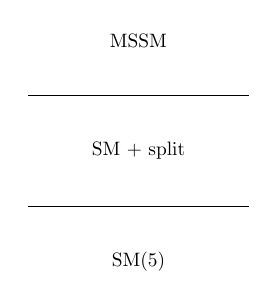
\begin{tikzpicture}[scale=0.7, every node/.style={transform shape}]
        \node at (2,4) {MSSM};
        \draw (0,3) -- (4,3);
        \node at (2,2) {SM + split};
        \draw (0,1) -- (4,1);
        \node at (2,0) {SM(5)};
      \end{tikzpicture}
    }{\footnotesize{II light $\chi_i$, $\tilde{g}$}}\hfill
    \stackunder[1em]{%
      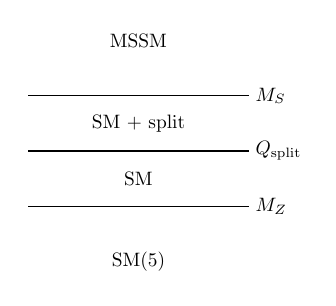
\begin{tikzpicture}[scale=0.7, every node/.style={transform shape}]
        \node at (2,4) {MSSM};
        \draw (0,3) -- (4,3) node[anchor=west] {$\MS$};
        \node at (2,2.5) {SM + split};
        \draw (0,2) -- (4,2) node[anchor=west] {$\Qsplit$};
        \node at (2,1.5) {SM};
        \draw (0,1) -- (4,1) node[anchor=west] {$M_Z$};
        \node at (2,0) {SM(5)};
      \end{tikzpicture}
    }{\footnotesize{III intermediate  $\chi_i$, $\tilde{g}$}}
  \end{figure}
\end{frame}

\begin{frame}{Scenarios with 2 light/intermediate Higgs doublets}
  \begin{figure}
    \centering
    \stackunder[1em]{%
      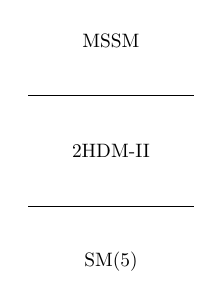
\begin{tikzpicture}[scale=0.7, every node/.style={transform shape}]
        \node at (1.5,4) {MSSM};
        \draw (0,3) -- (3,3);
        \node at (1.5,2) {2HDM-II};
        \draw (0,1) -- (3,1);
        \node at (1.5,0) {SM(5)};
      \end{tikzpicture}
    }{\footnotesize{IV light $h_i$, $A$, $H^{\pm}$}}\hfill
    \stackunder{%
    \stackunder[1em]{%
      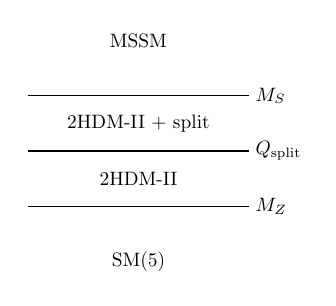
\begin{tikzpicture}[scale=0.7, every node/.style={transform shape}]
        \node at (2,4) {MSSM};
        \draw (0,3) -- (4,3) node[anchor=west] {$\MS$};
        \node at (2,2.5) {2HDM-II + split};
        \draw (0,2) -- (4,2) node[anchor=west] {$\Qsplit$};
        \node at (2,1.5) {2HDM-II};
        \draw (0,1) -- (4,1) node[anchor=west] {$M_Z$};
        \node at (2,0) {SM(5)};
      \end{tikzpicture}
    }{\footnotesize{V light $h_i$, $A$, $H^{\pm}$,}}}{\footnotesize{intermediate $\chi_i$, $\tilde{g}$}}\hfill
    \stackunder{%
    \stackunder[1em]{%
      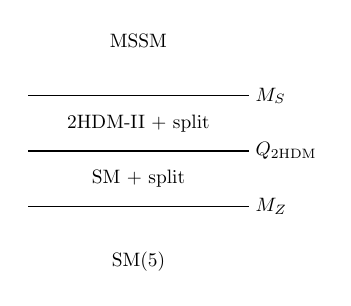
\begin{tikzpicture}[scale=0.7, every node/.style={transform shape}]
        \node at (2,4) {MSSM};
        \draw (0,3) -- (4,3) node[anchor=west] {$\MS$};
        \node at (2,2.5) {2HDM-II + split};
        \draw (0,2) -- (4,2) node[anchor=west] {$\QTHDM$};
        \node at (2,1.5) {SM + split};
        \draw (0,1) -- (4,1) node[anchor=west] {$M_Z$};
        \node at (2,0) {SM(5)};
      \end{tikzpicture}
    }{\footnotesize{VI light $h$, $\chi_i$, $\tilde{g}$,}}}{\footnotesize{intermediate $H$, $A$, $H^{\pm}$}}
  \end{figure}
\end{frame}

\section{Uncertainty estimate}

\begin{frame}{Contents}
  \tableofcontents[currentsection]  
\end{frame}

\begin{frame}{Considered sources of uncertainty}
\emph{SM/2HDM-II uncertainty}:
  \begin{align*}
    \Delta M_h^{(\SM)} &=
    \left| M_h(y_t^{(2L)}) - M_h(y_t^{(3L)}) \right|
                         + \max_{Q\in[M_t/2, 2M_t]}\left| M_h - M_h(Q) \right|
  \end{align*}
\emph{EFT uncertainty}:
  \begin{align*}
    \Delta M_h^{(\EFT)} = \left| M_h - M_h(\Delta\lambda_i \rightarrow \Delta\lambda_i [1 +
    v^2/\MS^2]) \right|
  \end{align*}
\emph{SUSY uncertainty}:
  \begin{align*}
    \Delta M_h^{(\MSSM)} = \left| M_h - M_h(y_t^{\EFT}(\MS) \rightarrow y_t^{\EFT}(\MS) [1 +
    \Delta y_t]) \right|
  \end{align*}
\emph{Parametric uncertainty}:
  \begin{align*}
    \Delta M_h^{(\text{par})} &= |M_h - M_h(M_t \pm \sigma_{M_t})|
                                + \left|M_h - M_h(\alpha_s(M_Z) \pm \sigma_{\alpha_s})\right|\\
    \sigma_{M_t} &= 0.98\eh{GeV}, \qquad
    \sigma_{\alpha_s} = 0.0006
  \end{align*}
\end{frame}

\begin{frame}{Combination of uncertainties}
  \emph{Combination:}
  \begin{align*}
    \Delta M_h = | \Delta M_h^{(\SM)} | + | \Delta M_h^{(\EFT)} |
    + | \Delta M_h^{(\MSSM)} | + | M_h^{(\text{par})} | .  
  \end{align*}
\end{frame}

\begin{frame}{Individual uncertainties in scenario IV (2HDM-II)}
  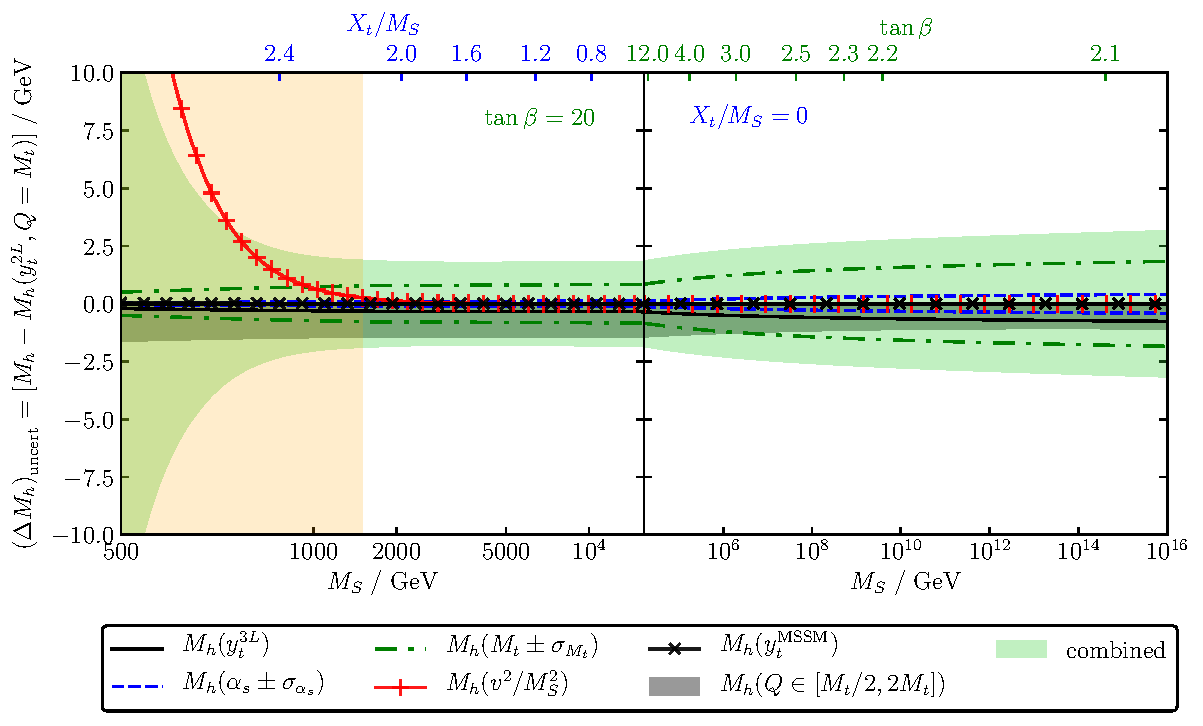
\includegraphics[width=\textwidth]{{{plots/THDM/THDMIIMSSMBCFull_uncertainty_MS_MA-800_uncertainty_advanced}}}
\end{frame}

\begin{frame}{Observations}
  For scenario IV (2HDM-II) in the studied range we find:
  \begin{itemize}
  \item Parametric uncertainty \emph{dominant}:
    \begin{align*}
      \Delta M_h(M_t \pm \sigma_{M_t}) &= (1\ldots 2)\eh{GeV} \\
      \Delta M_h(\alpha_s \pm \sigma_{\alpha_s}) &= (0.1\ldots 0.5)\eh{GeV}
    \end{align*}
  \item 2HDM-II uncertainty \emph{important}:
    \begin{align*}
      \Delta M_h(Q\in[M_t/2,2M_t]) &= (1\ldots 1.5)\eh{GeV}  ~~\text{(only 1L)} \\
      \Delta M_h(y_t^{2L}~\text{vs.}~y_t^{3L}) &= (0.3\ldots 0.5)\eh{GeV}
    \end{align*}
  \item EFT uncertainty $< 100\eh{MeV}$ for $\MS \gtrsim 2\eh{TeV}$
  \item SUSY uncertainty $< 10\eh{MeV}$ for $\MS \gtrsim 2\eh{TeV}$
  \end{itemize}
\end{frame}

\section{Results}

\begin{frame}{Contents}
  \tableofcontents[currentsection]  
\end{frame}

\begin{frame}{I high-scale SUSY}
  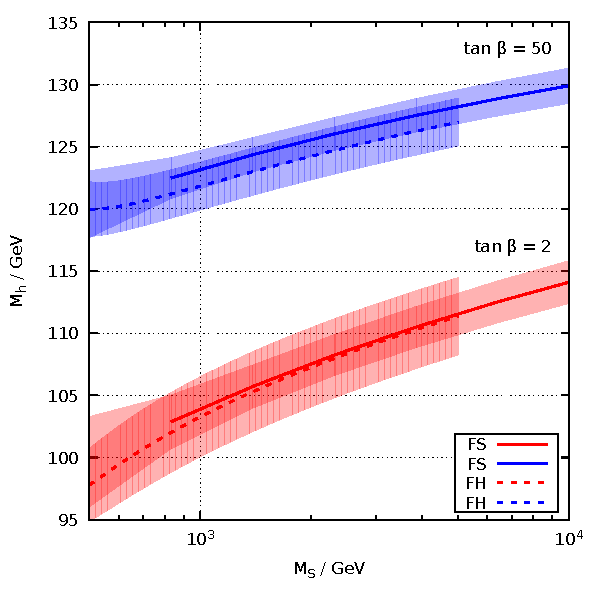
\includegraphics[width=0.49\textwidth]{{{plots/HSSUSY/HSSUSY_degenerate_Xt-2.44949_lowMSView}}}\hfill
  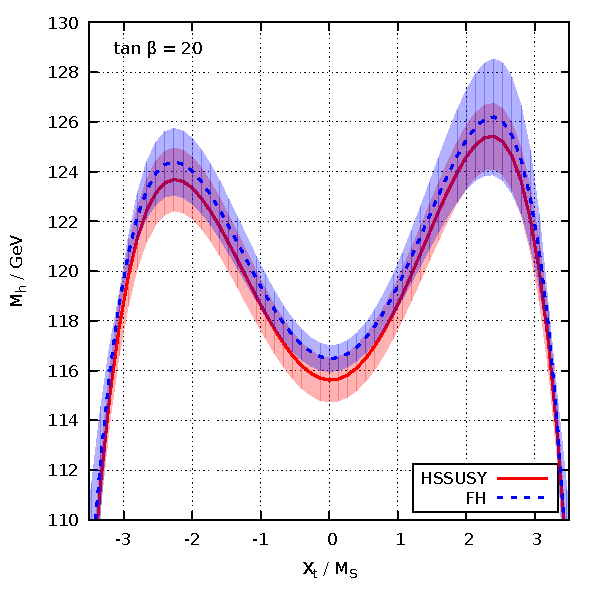
\includegraphics[width=0.49\textwidth]{{{plots/HSSUSY/HSSUSY_Xt_TB-20_MS-2000_talk}}}\\
  $X_t = \sqrt{6}\MS$, $\MS = 2\eh{TeV}$
\end{frame}

\begin{frame}{III intermediate  $\chi_i$, $\tilde{g}$}
  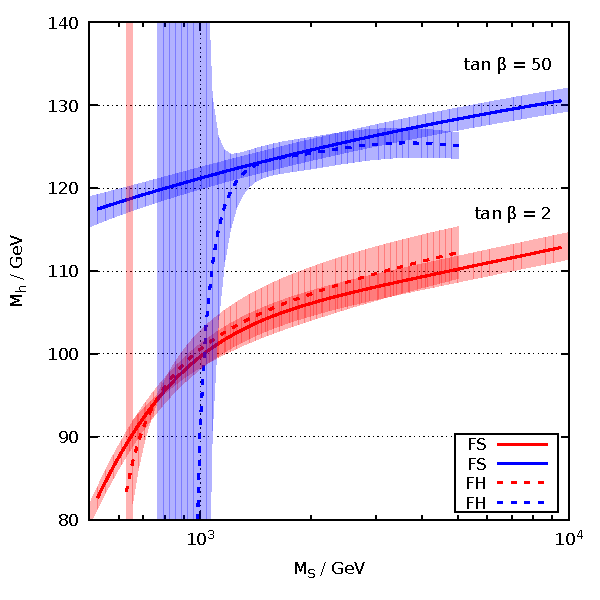
\includegraphics[width=0.49\textwidth]{{{plots/SplitMSSM/SplitMSSMTower_degenerate_Xt-2.44949_Mi-2000_lowMSView}}}\hfill
  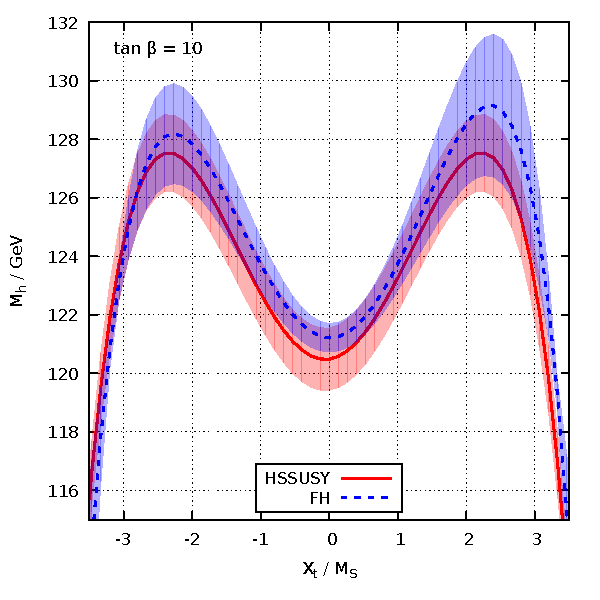
\includegraphics[width=0.49\textwidth]{{{plots/SplitMSSM/SplitMSSMTower_Xt_TB-10_MS-5000_Mi-2000_talk}}}\\
  $X_t = \sqrt{6}\MS$, $\MS = 2\eh{TeV}$, $M_i = \mu = 2\eh{TeV}$
\end{frame}

\begin{frame}{Effect from non-degenerate spectra}
  Variation of all SUSY mass parameters by factor 2:\\[1em]
  \stackunder[0.3em]{I high-scale SUSY}{%
    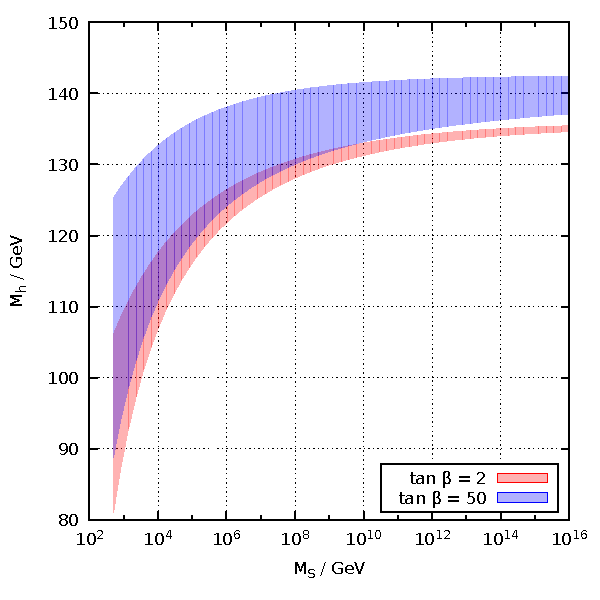
\includegraphics[width=0.49\textwidth]{{{plots/HSSUSY/HSSUSY_non_degenerate_talk}}}
  }\hfill
  \stackunder[0.3em]{II light $\chi_i$, $\tilde{g}$}{%
    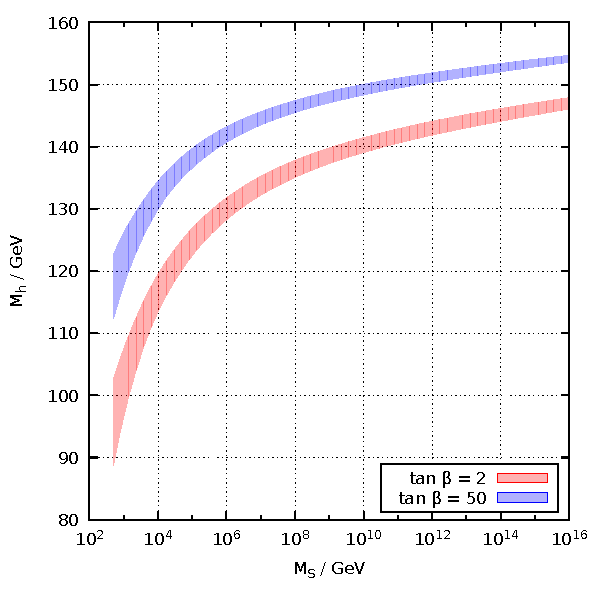
\includegraphics[width=0.49\textwidth]{{{plots/SplitMSSM/SplitMSSM_non_degenerate_talk}}}
  }\\
  $X_t = \sqrt{6}\MS$, $M_i^{\text{central}} = \mu^{\text{central}} = 2\eh{TeV}$
\end{frame}

\begin{frame}{IV light $h_i$, $A$, $H^{\pm}$}
  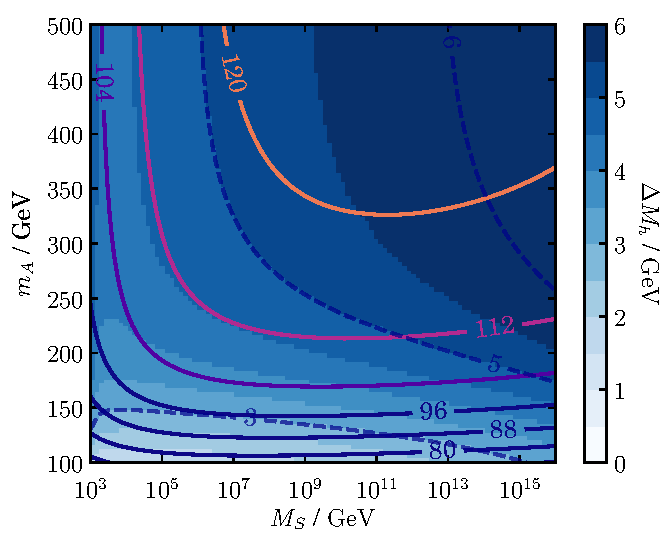
\includegraphics[width=0.49\textwidth]{{{plots/THDM/THDMIIMSSMBCFull_MS_MA_Xt-2.44949_TB-2}}}\hfill
  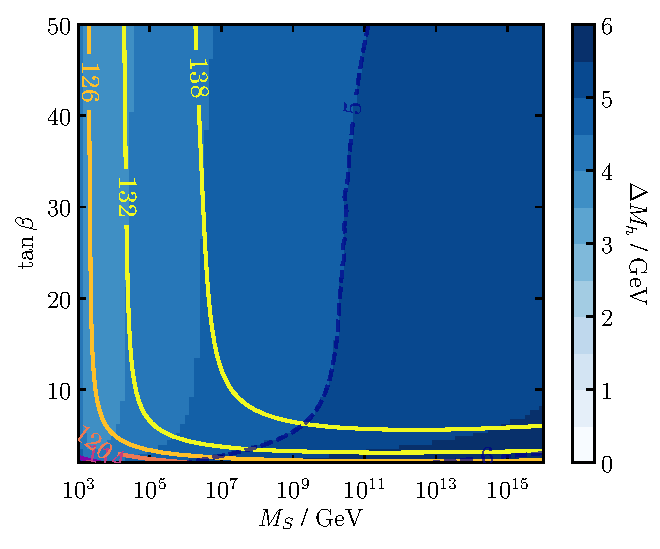
\includegraphics[width=0.49\textwidth]{{{plots/THDM/THDMIIMSSMBCFull_TB_MS_Xt-2.44949_MA-800}}}\\
  $X_t = \sqrt{6}\MS$\\ left: $\tan\beta = 2$, right: $m_A = 800\eh{GeV}$
\end{frame}

\begin{frame}{V light $h_i$, $A$, $H^{\pm}$, intermediate $\chi_i$, $\tilde{g}$}
  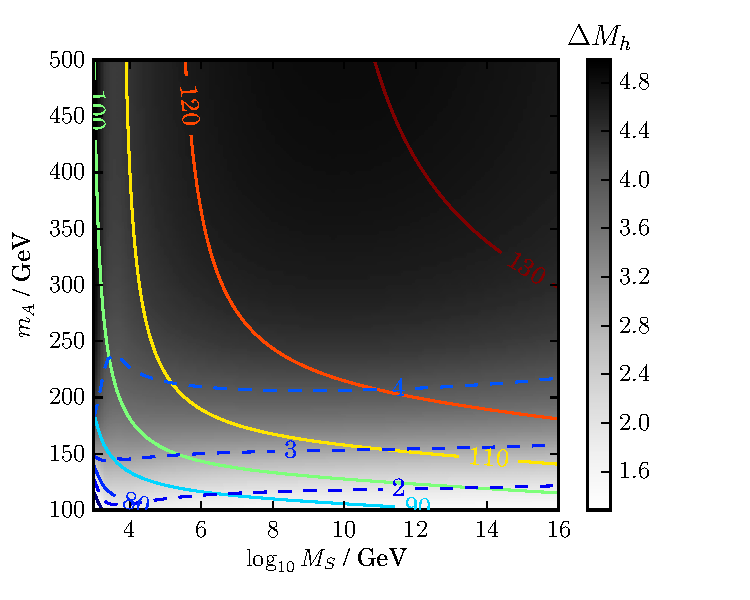
\includegraphics[width=0.49\textwidth]{{{plots/THDM/SplitTHDMTHDMTower_MS_MA_Xt-2.44949_TB-2_Mu-M12-M3-2000}}}\hfill
  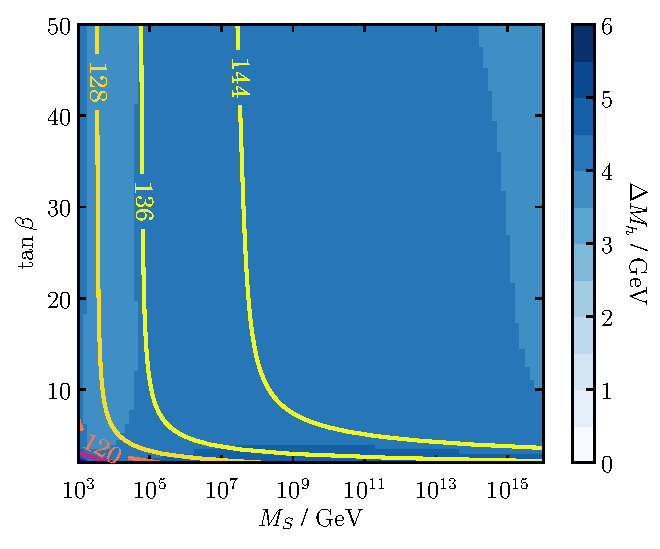
\includegraphics[width=0.49\textwidth]{{{plots/THDM/SplitTHDMTHDMTower_TB_MS_Xt-2.44949_MA-800_Mu-M12-M3-2000}}}\\
  $X_t = \sqrt{6}\MS$, $\mu = M_i = 2\eh{TeV}$\\
  left: $\tan\beta = 2$, right: $m_A = 800\eh{GeV}$
\end{frame}

\begin{frame}{VI light $h$, $\chi_i$, $\tilde{g}$, intermediate $H$, $A$, $H^{\pm}$}
  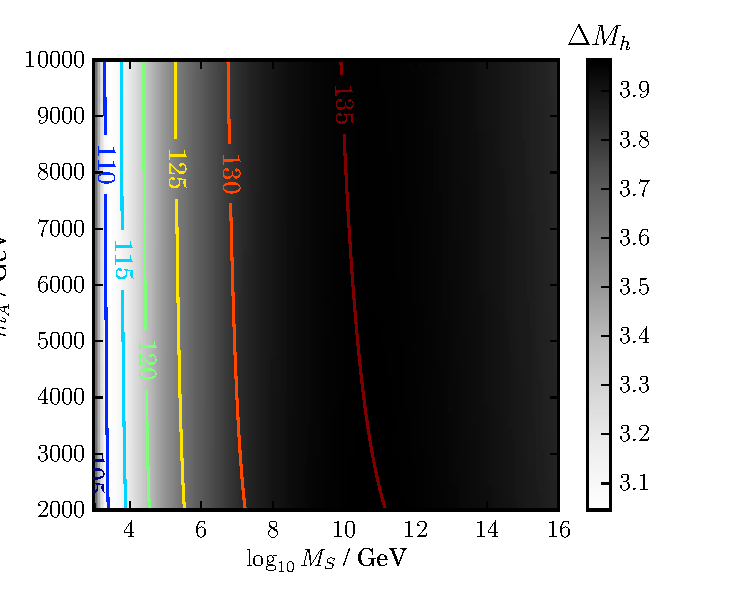
\includegraphics[width=0.49\textwidth]{{{plots/THDM/SplitTHDMSplitTower_MS_MA_Xt-2.44949_TB-2_Mu-M12-M3-1000}}}\hfill
  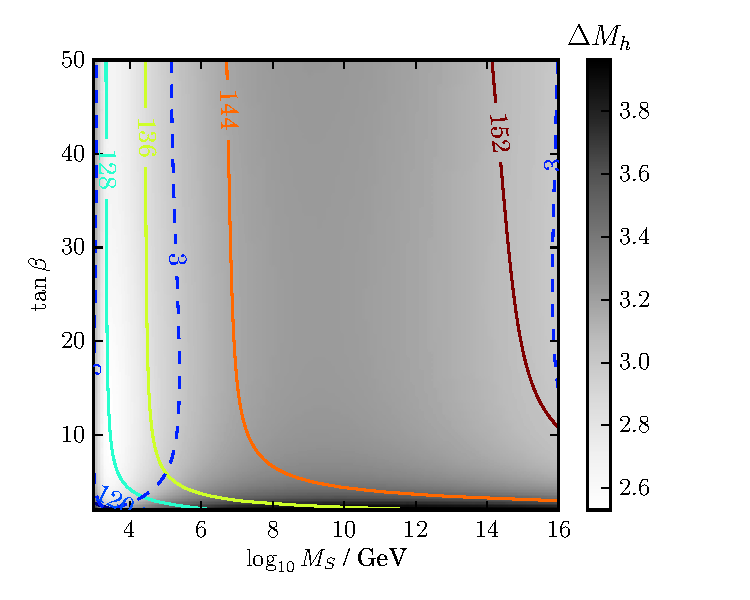
\includegraphics[width=0.49\textwidth]{{{plots/THDM/SplitTHDMSplitTower_TB_MS_Xt-2.44949_MA-2000_Mu-M12-M3-1000}}}\\
  $X_t = \sqrt{6}\MS$, $\mu = M_i = 1\eh{TeV}$\\
  left: $\tan\beta = 2$, right: $m_A = 2\eh{TeV}$
\end{frame}

%%%%%%%%%%%%%%%%%%%%%%%%%%%%%%%%%%%%%%%%

\begin{frame}{Summary}
  \begin{itemize}
  \item study 6 different mass hierarchies of the MSSM with FlexibleSUSY
  \item aim for honest uncertainty estimate\\ 4 sources:
    \begin{itemize}
    \item parametric uncertainty (dominant)
    \item SM/2HDM-II uncertainty (important, can be improved)
    \item EFT uncertainty (negligible, $< 100\eh{MeV}$ for $\MS \gtrsim 2\eh{TeV}$)
    \item SUSY uncertainty (negligible? $< 10\eh{MeV}$ for $\MS \gtrsim 2\eh{TeV}$)
    \end{itemize}
  \end{itemize}
\end{frame}

%%%%%%%%%%%%%%%%%%%%%%%%%%%%%%%%%%%%%%%%
% backup slides
%%%%%%%%%%%%%%%%%%%%%%%%%%%%%%%%%%%%%%%%

\begin{frame}[noframenumbering]
  \begin{center}
    \Huge Backup
  \end{center}
\end{frame}

\begin{frame}[noframenumbering]{I high-scale SUSY}
  \emph{Input parameters:}
  \begin{align*}
  \tan\beta^{\DRbar}(\MS), A_t^{\DRbar}(\MS), m_A^{\DRbar}(\MS),
  \mu^{\DRbar}(\MS), M_i^{\DRbar}(\MS),
  (m_{\tilde{f}}^2)^{\DRbar}_{ij}(\MS)
  \end{align*}
  \emph{Threshold correction:}
  \begin{align*}
    \lambda(\MS) &= \frac{1}{4}\left(\frac{3}{5} g_1^2 +
                   g_2^2\right) \cos^22\beta + \DlHSSUSY{1} + \DlHSSUSY{2}
  \end{align*}
  \hfill\bigcite{1407.4081, 1703.08166}
\end{frame}

\begin{frame}[noframenumbering]{II light $\chi_i$, $\tilde{g}$}
\begin{align*}
  \Lag_{\SplitMSSM} &= \Lag_{\SM} + \Lag_\text{split}, \\
\begin{split}
  \Lag_\text{split} \supset
  &- \frac{M_1}{2} \tilde{B}\tilde{B}
  - \frac{M_2}{2} \tilde{W}^i\tilde{W}^i
  - \frac{M_3}{2} \tilde{g}^a\tilde{g}^a
  - \mu \tilde{H}_u\cdot \tilde{H}_d \\
  &-\frac{H^\dagger}{\sqrt{2}} \left(
    \gSplitMSSM{2u} \sigma^i\tilde{W}^i + \gSplitMSSM{1u} \tilde{B}
  \right)\tilde{H}_u \\
  &-\frac{H}{\sqrt{2}} \cdot  \left(
    -\gSplitMSSM{2d} \sigma^i\tilde{W}^i + \gSplitMSSM{1d} \tilde{B}
  \right) \tilde{H}_d
  + \hc
\end{split}
\end{align*}
\end{frame}

\begin{frame}[noframenumbering]{II light $\chi_i$, $\tilde{g}$}
  \emph{Input parameters:}
  \begin{align*}
    \tan\beta^{\DRbar}(\MS), A_t^{\DRbar}(\MS), m_A^{\DRbar}(\MS),
    \mu^{\MSbar}(M_Z), M_i^{\MSbar}(M_Z),
    (m_{\tilde{f}}^2)^{\DRbar}_{ij}(\MS)
  \end{align*}
  \emph{Threshold correction:}
  \begin{align*}
    \tilde\lambda(\MS) &= \frac{1}{4}\left(\frac{3}{5} g_1^2 + g_2^2\right)
    \cos^22\beta + \DlSplitMSSM{1} + \DlSplitMSSM{2} ,\\
    \gSplitMSSM{1u}(\MS) &= \sqrt{\frac{3}{5}} g_1 \sin\beta + \DgSplitMSSM{1u},\\
    \gSplitMSSM{1d}(\MS) &= \sqrt{\frac{3}{5}} g_1 \cos\beta + \DgSplitMSSM{1d},\\
    \gSplitMSSM{2u}(\MS) &= g_2 \sin\beta + \DgSplitMSSM{2u},\\
    \gSplitMSSM{2d}(\MS) &= g_2 \cos\beta + \DgSplitMSSM{2d}
  \end{align*}
  \hfill\bigcite{1407.4081}
\end{frame}

\begin{frame}[noframenumbering]{III intermediate  $\chi_i$, $\tilde{g}$}
  \emph{Input parameters:}
  \begin{align*}
  \tan\beta^{\DRbar}(\MS), A_t^{\DRbar}(\MS), m_A^{\DRbar}(\MS),
  \mu^{\MSbar}(\Qsplit), M_i^{\MSbar}(\Qsplit),
  (m_{\tilde{f}}^2)^{\DRbar}_{ij}(\MS)
  \end{align*}
  \emph{Threshold correction:}
  \begin{align*}
  \lambda(\Qsplit) &= \tilde\lambda(\Qsplit) + \Delta\lambda^{\text{1L,}\chi^1} \\
  y_t^\SplitMSSM(\Qsplit) &= y_t^\SM(\Qsplit) (1 + \Delta g_t^\chi) \\
  g_i^\SplitMSSM(\Qsplit) &= g_i^\SM(\Qsplit) (1 + \Delta g_i)
  \end{align*}
  \hfill\bigcite{1407.4081}
\end{frame}

\begin{frame}[noframenumbering]{IV light $h_i$, $A$, $H^{\pm}$}
\begin{align*}
\begin{split}
  \Lag_\THDM \supset
  &-m_1^2 |H_1|^2 + m_2^2 |H_2|^2
  - \lambda_1 (H_1^\dagger H_1)^2
  - \lambda_2 (H_2^\dagger H_2)^2 \\
  &- \lambda_3 |H_1|^2 |H_2|^2
  - \lambda_4 |H_2^\dagger H_1|^2\\
  &+\Bigg[ m_{12}^2 H_1^\dagger H_2
  - \frac{\lambda_5}{2} (H_1^\dagger H_2)^2
  - \lambda_6 (H_1^\dagger H_1)(H_1^\dagger H_2)\\
  &\qquad- \lambda_7 (H_2^\dagger H_2)(H_1^\dagger H_2)
  + \hc \Bigg] .
\end{split}
\end{align*}
\end{frame}

\begin{frame}[noframenumbering]{IV light $h_i$, $A$, $H^{\pm}$}
  \emph{Input parameters:}
  \begin{align*}
  \tan\beta^{\MSbar}(M_t), A_t^{\DRbar}(\MS), m_A^{\MSbar}(M_t),
  \mu^{\DRbar}(\MS), M_i^{\DRbar}(\MS),
  (m_{\tilde{f}}^2)^{\DRbar}_{ij}(\MS)
  \end{align*}
  \emph{Threshold correction:}
  \begin{align*}
    \lambda_1(\MS) &= \frac{1}{4}\left(\frac{3}{5} g_1^2 + g_2^2\right) + \DlTHDM{1}{1} + \DlTHDM{1}{2}\\
    \lambda_2(\MS) &= \frac{1}{4}\left(\frac{3}{5} g_1^2 + g_2^2\right) + \DlTHDM{2}{1} + \DlTHDM{2}{2}\\
    \lambda_3(\MS) &= -\frac{1}{4} \left(\frac{3}{5}g_1^2 + g_2^2\right) + \frac{g_2^2}{2} + \DlTHDM{3}{1} + \DlTHDM{3}{2}\\
    \lambda_4(\MS) &= -\frac{g_2^2}{2} + \DlTHDM{4}{1} + \DlTHDM{4}{2}\\
    \lambda_5(\MS) &= 0 + \DlTHDM{5}{1} + \DlTHDM{5}{2}\\
    \lambda_6(\MS) &= 0 + \DlTHDM{6}{1} + \DlTHDM{6}{2}\\
    \lambda_7(\MS) &= 0 + \DlTHDM{7}{1} + \DlTHDM{7}{2}
  \end{align*}
  \hfill\bigcite{0901.2065, 1508.00576}
\end{frame}

\begin{frame}[noframenumbering]{V light $h_i$, $A$, $H^{\pm}$, intermediate $\chi_i$, $\tilde{g}$}
\begin{align*}
  \Lag_{\SplitTHDM} &= \Lag_{\THDM} + \Lag_\text{split}, \\
\begin{split}
  \Lag_\text{split} \supset
  &- \frac{M_1}{2} \tilde{B}\tilde{B}
  - \frac{M_2}{2} \tilde{W}^i\tilde{W}^i
  - \frac{M_3}{2} \tilde{g}^a\tilde{g}^a
  - \mu \tilde{H}_u\cdot \tilde{H}_d \\
  &-\frac{H_2^\dagger}{\sqrt{2}} \left( \gSplitTHDM{2u} \sigma^i\tilde{W}^i
     +\gpSplitTHDM{2u} \tilde{B} \right)\tilde{H}_u \\
  &-\frac{H_1}{\sqrt{2}} \cdot  \left( -\gSplitTHDM{1d} \sigma^i\tilde{W}^i
     + \gpSplitTHDM{1d} \tilde{B} \right) \tilde{H}_d
  + \hc
\end{split}
\end{align*}
\end{frame}

\begin{frame}[noframenumbering]{V light $h_i$, $A$, $H^{\pm}$, intermediate $\chi_i$, $\tilde{g}$}
  \emph{Input parameters:}
  \begin{align*}
  \tan\beta^{\MSbar}(M_t), A_t^{\DRbar}(\MS), m_A^{\MSbar}(M_t),
  \mu^{\MSbar}(\Qsplit), M_i^{\MSbar}(\Qsplit),
  (m_{\tilde{f}}^2)^{\DRbar}_{ij}(\MS)
  \end{align*}
  \emph{Threshold correction:}
  \begin{align*}
    \tilde\lambda_1 &= \frac{1}{4}\left(\frac{3}{5} g_1^2 + g_2^2\right) + \DlSplitTHDM{1}{1} + \DlSplitTHDM{1}{2},\\
    \tilde\lambda_2 &= \frac{1}{4}\left(\frac{3}{5} g_1^2 + g_2^2\right) + \DlSplitTHDM{2}{1} + \DlSplitTHDM{2}{2},\\
    \tilde\lambda_3 &= -\frac{1}{4} \left(\frac{3}{5}g_1^2 + g_2^2\right) + \frac{g_2^2}{2} + \DlSplitTHDM{3}{1} + \DlSplitTHDM{3}{2},\\
    \tilde\lambda_4 &= -\frac{g_2^2}{2} + \DlSplitTHDM{4}{1} + \DlSplitTHDM{4}{2},\\
    \tilde\lambda_i &= 0 + \DlSplitTHDM{i}{1} + \DlSplitTHDM{i}{2}, \quad (i = 5,6,7)\\
    \gpSplitTHDM{1d} &= \sqrt{\frac{3}{5}} g_1, \qquad
    \gSplitTHDM{1d}  = g_2, \qquad
    \gpSplitTHDM{2u} = \sqrt{\frac{3}{5}} g_1, \qquad
    \gSplitTHDM{2u}  = g_2
  \end{align*}
  \hfill\bigcite{0901.2065, 1508.00576}
\end{frame}

\begin{frame}[noframenumbering]{VI light $h$, $\chi_i$, $\tilde{g}$, intermediate $H$, $A$, $H^{\pm}$}
  \emph{Input parameters:}
  \begin{align*}
  \tan\beta^{\MSbar}(\QTHDM), A_t^{\DRbar}(\MS), m_A^{\MSbar}(\QTHDM),
  \mu^{\MSbar}(M_Z), M_i^{\MSbar}(M_Z),
  (m_{\tilde{f}}^2)^{\DRbar}_{ij}(\MS)
  \end{align*}
  \emph{Threshold correction:}
  \begin{align*}
    \begin{split}
      \tilde\lambda &= 2 \tilde\lambda_1 c_\beta^4 + 2
      \tilde\lambda_2 s_\beta^4
      + 2 \left(\tilde\lambda_3 +
        \tilde\lambda_4 +
        \tilde\lambda_5 \right) c_\beta^2 s_\beta^2
      + 4 \tilde\lambda_6 c_\beta^3 s_\beta + 4
      \tilde\lambda_7 c_\beta s_\beta^3 \\
      &\phantom{=\;} + \Delta\lambda^{\SplitTHDM-\SplitMSSM},
    \end{split} \\
    \mu^{\SplitMSSM} &= \mu^{\SplitTHDM}, \\
    M_i^{\SplitMSSM} &= M_i^{\SplitTHDM}, \\
    \gSplitMSSM{1u} &= \gpSplitTHDM{2u} \sin\beta + \DgSplitTHDMSplit{1u},\\
    \gSplitMSSM{1d} &= \gpSplitTHDM{1d} \cos\beta + \DgSplitTHDMSplit{1d},\\
    \gSplitMSSM{2u} &= \gSplitTHDM{2u} \sin\beta + \DgSplitTHDMSplit{2u},\\
    \gSplitMSSM{2d} &= \gSplitTHDM{1d} \cos\beta + \DgSplitTHDMSplit{2d}.
  \end{align*}
  \hfill\bigcite{0901.2065, 1508.00576}
\end{frame}

\begin{frame}[noframenumbering]{Determination of MSSM parameters}
  \emph{Fixed by observables:}
  \begin{table}
    \centering
    \begin{tabular}{lllll}
      Input & & & & Output \\
      \midrule
      $\alpha_\text{em}^{\SM(5)}(M_Z)$ & $\rightarrow$ & $\alpha_\text{em}^\MSSM(M_Z)$ & $\rightarrow$ & $g_1^\MSSM(M_Z)$ \\
      $G_F$ & $\rightarrow$ & $\sin\theta_W^\MSSM(M_Z)$ & $\rightarrow$ & $g_2^\MSSM(M_Z)$ \\
      $\alpha_\text{s}^{\SM(5)}(M_Z)$ & & & $\rightarrow$ & $g_3^\MSSM(M_Z)$ \\
      $M_Z$ & $\rightarrow$ & $m_Z^\MSSM(M_Z)$ & $\rightarrow$ & $v^\MSSM(M_Z)$ \\
      $M_t$ & $\rightarrow$ & $m_t^\MSSM(M_Z)$ & $\rightarrow$ & $y_t^\MSSM(M_Z)$ \\
      $m_b^{\SM(5)}(m_b)$ & $\rightarrow$ & $m_b^\MSSM(M_Z)$ & $\rightarrow$ & $y_b^\MSSM(M_Z)$ \\
      $M_\tau$ & $\rightarrow$ & $m_\tau^\MSSM(M_Z)$ & $\rightarrow$ & $y_\tau^\MSSM(M_Z)$ \\
    \end{tabular}
  \end{table}
  \emph{Fixed by 2 EWSB conditions:} $m^2_{H_u}$, $m^2_{H_d}$ \\[1em]
  \emph{Free parameters:} $\tan\beta$, $\mu$, $B\mu$, $m_{\tilde{f},ij}^2$, $M_i$,
  $T^f_{ij}$
\end{frame}

\begin{frame}[noframenumbering]{Determination of SM parameters}
  \emph{Fixed by observables:}
  \begin{table}
    \centering
    \begin{tabular}{lllll}
      Input & & & & Output \\
      \midrule
      $\alpha_\text{em}^{\SM(5)}(M_Z)$ & $\rightarrow$ & $\alpha_\text{em}^\SM(M_Z)$ & $\rightarrow$ & $g_1^\SM(M_Z)$ \\
      $G_F$ & $\rightarrow$ & $\sin\theta_W^\SM(M_Z)$ & $\rightarrow$ & $g_2^\SM(M_Z)$ \\
      $\alpha_\text{s}^{\SM(5)}(M_Z)$ & & & $\rightarrow$ & $g_3^\SM(M_Z)$ \\
      $M_Z$ & $\rightarrow$ & $m_Z^\SM(M_Z)$ & $\rightarrow$ & $v^\SM(M_Z)$ \\
      $M_t$ & $\rightarrow$ & $m_t^\SM(M_Z)$ & $\rightarrow$ & $y_t^\SM(M_Z)$ \\
      $m_b^{\SM(5)}(m_b)$ & $\rightarrow$ & $m_b^\SM(M_Z)$ & $\rightarrow$ & $y_b^\SM(M_Z)$ \\
      $M_\tau$ & $\rightarrow$ & $m_\tau^\SM(M_Z)$ & $\rightarrow$ & $y_\tau^\SM(M_Z)$ \\
    \end{tabular}
  \end{table}
  \emph{Fixed by 1 EWSB condition:} $\mu^2$ \\[1em]
  \emph{Free parameter:} $\lambda$
\end{frame}

% \subsubsection{Determination of MSSM parameters}

% \begin{frame}
%   \tableofcontents[currentsection]  
% \end{frame}

\begin{frame}[noframenumbering]{Determination of $g_3^\MSSM(M_S)$}
  \begin{align*}
    \alpha_{\text{s}}^{\MSSM}(M_S) &=
    \frac{\alpha_{\text{s}}^{\SM}(M_S)}{1 -
      \Delta\alpha_{\text{s}}(M_S)} \intertext{with}
    \Delta\alpha_{\text{s}}(Q) &= \frac{\alpha_\text{s}}{2\pi}\left[
      \frac{1}{2}-\sum_{\text{SUSY particle } f} T_f
      \log{\frac{m_f}{Q}} \right] \intertext{$\Rightarrow$}
    g_{3}^{\MSSM}(M_S) &= \sqrt{4\pi\alpha_{\text{s}}^{\MSSM}(M_S)}
  \end{align*}
\end{frame}

\begin{frame}[noframenumbering]{Determination of $v_i^\MSSM(M_S)$}
  \begin{align*}
    M_Z^\SM = M_Z^\MSSM
  \end{align*}
  $\Rightarrow$
  \begin{align*}
    (m_Z^{\MSSM}(M_S))^2 &= (M_Z^\SM)^2 + \Pi_Z^{\MSSM,1L}(Q=M_S) \\
    (M_Z^{\SM})^2 &= \frac{1}{4} \left[(g_Y^\SM)^2 + (g_2^\SM)^2\right] (v^\SM)^2 - \Pi_Z^{\SM,1L}(Q=M_S)
  \end{align*}
  $\Rightarrow$
  \begin{align*}
    v^\MSSM(M_S) &= \frac{2 m_Z^{\MSSM}(M_S)}{\sqrt{(g_Y^\MSSM)^2 + (g_2^\MSSM)^2}}
    \intertext{$\Rightarrow$}
    v_u^{\MSSM}(M_S) &= v^\MSSM(M_S) \sin\beta(M_S) \\
    v_d^{\MSSM}(M_S) &= v^\MSSM(M_S) \cos\beta(M_S)
  \end{align*}
\end{frame}

\begin{frame}[noframenumbering]{Determination of $y_i^\MSSM(M_S)$}
  \begin{align*}
    M_f^\SM = M_f^\MSSM
  \end{align*}
  $\Rightarrow$
  \begin{align*}
    m_f^{\MSSM}(M_S) &= M_f^\SM + \Sigma_f^{\MSSM,1L}(Q=M_S) \\
    M_f^{\SM} &= \frac{\sqrt{2} m_f^\SM}{v_i^\SM} - \Sigma_f^{\SM,1L}(Q=M_S)
  \end{align*}
  $\Rightarrow$
  \begin{align*}
    y_f^\MSSM(M_S) = \frac{\sqrt{2} m_f^\MSSM(M_S)}{v_i^\MSSM(M_S)}
  \end{align*}
\end{frame}

%%%%%%%%%%%%%%%%%%%%%%%%%%%%%%%%%%%%%%%%%%

\begin{frame}[noframenumbering]
  \begin{center}
    \Large Determination of SM parameters
  \end{center}
\end{frame}

\begin{frame}[noframenumbering]{Determination of $g_3^{\SM}(M_Z)$}
  \emph{Input:} \ \ $\alpha_{\text{s}}^{\SM(5)}(M_Z) = 0.1185$\\[1em]
  $\rightarrow$
  \begin{align*}
    \alpha_{\text{s}}^{\SM}(M_Z) &=
    \frac{\alpha_{\text{s}}^{\SM(5)}(M_Z)}{1 -
      \Delta\alpha_{\text{s}}(M_Z)} \intertext{with}
    \Delta\alpha_{\text{s}}(Q) &=
    \frac{\alpha_\text{s}}{2\pi} \left[
      -\frac{2}{3} \log{\frac{m_t}{Q}} \right]
    \intertext{$\Rightarrow$}
    g_{3}^{\SM}(M_Z) &=
    \sqrt{4\pi\alpha_{\text{s}}^{\SM}(M_Z)}
  \end{align*}
\end{frame}

\begin{frame}[noframenumbering]{Determination of $y_t^{\SM}(M_Z)$}
  \begin{align*}
    y_t^{\SM}(M_Z) &= \frac{\sqrt{2}\, m_{t}^{\SM}(M_Z)}{v(M_Z)}
    %
    \intertext{where}
    %
    m_{t}^{\SM}(Q) &= M_t +
    \re\Sigma_{t}^{S}(M_Z) + M_t \Big[ \re\Sigma_{t}^{L}(M_Z) \\
    &\phantom{={}} +
    \re\Sigma_{t}^{R}(M_Z) + \Delta
    m_t^{1L,\text{gluon}} + \Delta m_t^{2L,\text{gluon}} \Big]\\
    % m_{t}^{\text{\MSbar}} &= M_t +
    % \Sigma_{t}^\text{no gluon}(M_Z) + M_t \Big[\Delta
    % m_t^{(1L),\text{gluon}} + \Delta m_t^{(2L),\text{gluon}} \Big]
    % \\
    \Delta m_t^{1L,\text{gluon}} &= -\frac{g_3^2}{12 \pi^2}
    \left[4 - 3 \log\left(\frac{m_t^2}{Q^2}\right)\right]
    \\
    \Delta m_t^{2L,\text{gluon}} &= \left(\Delta
      m_t^{1L,\text{gluon}}\right)^2 \\
    &\phantom{=\;} - \frac{g_3^4}{4608 \pi^4} \Bigg[396
    \log^2\left(\frac{m_t^2}{Q^2}\right)
    - 1452 \log\left(\frac{m_t^2}{Q^2}\right) \\
    &\phantom{=\; - \frac{g_3^4}{4608 \pi^4}\Bigg[} -48
    \zeta(3)+2053+16 \pi ^2 (1+\log 4)\Bigg]
  \end{align*}
  $\Rightarrow$
\end{frame}

\begin{frame}[noframenumbering]{Determination of $v^\SM$}
  The VEV $v^\SM$ is calculated from the running $Z$ mass at $Q = M_Z$:
  \begin{align*}
    v^{\SM}(M_Z) &= \frac{2 m_Z^{\SM}(M_Z)}{\sqrt{g_Y^2 + g_2^2}} \\
    m_Z^{\SM}(M_Z) &= \sqrt{M_Z^2 + \Pi_Z^{1L}(p^2=M_Z^2,Q=M_Z)}
  \end{align*}
  $v^{\SM}$ evolves under RG running according to\\\bigcite{Sperling,
    Stöckinger, AV, 2013, 2014}
\end{frame}

%%%%%%%%%%%%%%%%%%%%%%%%%%%%%%%%%%%%%%%%%%%%%%

\begin{frame}[noframenumbering]{Comparison full model vs.\ EFT approach}
  \begin{center}
    Q: Why is FlexibleSUSY/MSSM so close to the EFT approaches and
    SPheno so far off?
  \end{center}
\end{frame}

\begin{frame}[noframenumbering]{Calculation of $y_t^{\text{MSSM}}(M_Z)$}
  A: Different treatment of 2-loop corrections to $y_t^{\text{MSSM}}(M_Z)$:
  \\[1em]
  \emph{FlexibleSUSY:}
  \begin{align*}
    m_t &=
    M_t+\re\left[
      \widetilde{\Sigma}_t^{(1),S}(M_t)\right] +
    \textcolor{red}{M_t} \re\left[
      \widetilde{\Sigma}_t^{(1),L}(M_t) +
      \widetilde{\Sigma}_t^{(1),R}(M_t)
    \right] \nonumber \\
    &\phantom{={}} + M_t
    \left[\widetilde{\Sigma}_t^{(1),\text{qcd}}(m_t)
      + \left(\widetilde{\Sigma}_t^{(1),\text{qcd}}(m_t)\right)^2
      + \widetilde{\Sigma}_t^{(2),\text{qcd}}(m_t)\right]
  \end{align*}
  \emph{SPheno:}
  \begin{align*}
    m_t &=
    M_t+\re\left[
      \widetilde{\Sigma}_t^{(1),S}(m_t)\right]+
    \textcolor{red}{m_t} \re\left[
      \widetilde{\Sigma}_t^{(1),L}(m_t) +
      \widetilde{\Sigma}_t^{(1),R}(m_t)
    \right] \nonumber \\
    &\phantom{={}} +
    m_t
    \left[\widetilde{\Sigma}_t^{(1),\text{qcd}}(m_t) +
      \widetilde{\Sigma}_t^{(2),\text{qcd}}(m_t)
    \right]
  \end{align*}
\end{frame}

\newcommand{\FS}{FlexibleSUSY\xspace}
\newcommand{\SARAH}{SARAH\xspace}
\newcommand{\Softsusy}{SOFTSUSY\xspace}
\newcommand{\SPheno}{SPheno\xspace}
\newcommand{\SUSYHD}{SUSYHD\xspace}

\newcommand{\bgsgs}{\beta_{\gshigh,\gshigh^2}}
\newcommand{\bytgs}{\beta_{\ythigh,\gshigh^2}}
\newcommand{\bytyt}{\beta_{\ythigh,\ythigh^2}}
\newcommand{\bvyt}{\beta_{\vhigh,\ythigh^2}}
\newcommand{\blambdaytyt}{\beta_{\lambdahigh,\ythigh^4}}
\newcommand{\blambdayt}{\beta_{\lambdahigh,\ythigh^2\lambdahigh}}
\newcommand{\blambdalambda}{\beta_{\lambdahigh,\lambdahigh^2}}
\newcommand{\btildegsgs}{\tilde\beta_{\gshigh,\gshigh^2}}
\newcommand{\btildeytgs}{\tilde\beta_{\ythigh,\gshigh^2}}
\newcommand{\btildeytyt}{\tilde\beta_{\ythigh,\ythigh^2}}
\newcommand{\btildevyt}{\tilde\beta_{\vhigh,\ythigh^2}}

\newcommand{\gs}{\hat{g}_3}
\newcommand{\gsMSSM}{\bar{g}_3}
\newcommand{\ytlow}{\hat{y}_t}
\newcommand{\ytMSSMlow}{\bar{y}_t}
\newcommand{\vlow}{\hat{v}}
\newcommand{\vMSSM}{\bar{v}}
\newcommand{\gshigh}{{g}_3}
\newcommand{\gsMSSMhigh}{\tilde{g}_3}
\newcommand{\ythigh}{y_t}
\newcommand{\ytMSSMhigh}{\tilde{y}_t}
\newcommand{\vhigh}{v}
\newcommand{\vMSSMhigh}{\tilde{v}}
\newcommand{\lambdalow}{\hat{\lambda}}
\newcommand{\lambdahigh}{{\lambda}}

\newcommand{\kappaL}{\kappa}

\begin{frame}[noframenumbering]{Calculation of $y_t^{\text{MSSM}}(M_Z)$}
  $\Rightarrow$
  \begin{align*}
    \ytMSSMhigh^{\text{\FS}} &= 
    \ythigh +
    t^2\kappaL^2 \left(\frac{184}{9} \gshigh^4 \ythigh -24 \gshigh^2
      \ythigh^3 
      +\frac{9}{8} \ythigh^5 \right) 
    +\ldots\\
    \ytMSSMhigh^{\text{\SPheno}} &= 
    \ythigh +
    t^2 \kappaL^2 \left(\frac{248}{9} \gshigh^4 \ythigh-16 \gshigh^2
      \ythigh^3
      +\frac{27}{8} \ythigh^5\right) 
    +\ldots
  \end{align*}
  with
  \begin{align*}
    y_t &\equiv y_t^\SM(M_S), & g_3 &\equiv g_3^\SM(M_S), \\
    \tilde{y}_t &\equiv y_t^\text{MSSM}(M_S), & \tilde{g}_3 &\equiv g_3^\text{MSSM}(M_S), \\
    t &\equiv \log\frac{M_S}{M_t}, & \kappaL &\equiv \frac{1}{(4 \pi)^2}
  \end{align*}
\end{frame}

\begin{frame}[noframenumbering]{Calculation of $y_t^{\text{MSSM}}(M_Z)$}
  \begin{align*}
    (M_h^2)^{\text{EFT}}&=
    m_h^2
    + \vhigh^2 
    \ythigh^4\Big[12 t \kappaL
    +12 t^2 \kappaL^2 
    \left(16 \gshigh^2 - 9\ythigh^2 \right)
    \\&\quad{}
    +
    4 t^3\kappaL^3  \left(736 \gshigh^4-672 \gshigh^2 \ythigh^2+90
      \ythigh^4\right) 
    +\ldots\Big],
    \\
    (M_h^2)^{\text{\FS}}&=
    m_h^2
    + \vhigh^2 
    \ythigh^4\Big[12 t \kappaL
    +12 t^2 \kappaL^2 
    \left(16 \gshigh^2 - 9\ythigh^2 \right)
    \\&\quad{}
    +4 t^3\kappaL^3 \left(\frac{736 \gshigh^4}{3}-288 \gshigh^2
      \ythigh^2+\frac{27 \ythigh^4}{2}\right)
    +\ldots\Big],
    \\
    (M_h^2)^{\text{\SPheno}}&=
    m_h^2
    + \vhigh^2 
    \ythigh^4\Big[12 t \kappaL
    +12 t^2 \kappaL^2 
    \left(16 \gshigh^2 - 9\ythigh^2 \right)
    \\&\quad{}
    +4 t^3\kappaL^3 \left(\frac{992 \gshigh^4}{3}-192 \gshigh^2
      \ythigh^2+\frac{81 \ythigh^4}{2}\right)
    +\ldots\Big].
  \end{align*}
\end{frame}

\end{document}
